\subsection{Edge-device implementation}
\label{sec:implementation}

The detectors are deployed in an iOS application written in Swift with
SwiftUI, which runs entirely on the device and needs no network connection.
Figure~\ref{fig:pipeline} shows the path from a trained checkpoint to a count
on the screen.

\begin{figure*}[t]
  \centering
  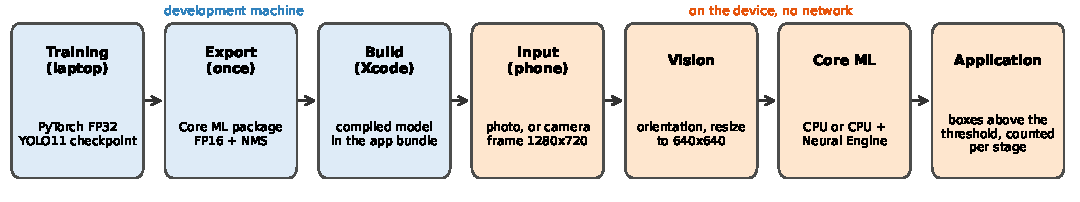
\includegraphics[width=\textwidth]{pipeline.pdf}
  \caption{From training to an on-device count. A PyTorch checkpoint is
  exported once to an FP16 Core ML package that already contains NMS; Xcode
  compiles it into the application; at run time the Vision framework resizes
  each photo or camera frame, Core ML runs the network on the CPU or on the
  Neural Engine, and the application counts the returned boxes per maturity
  stage.}
  \label{fig:pipeline}
\end{figure*}

\textbf{Export.} Each trained checkpoint is converted with the Ultralytics
exporter to a Core ML package in 16-bit floating point, which halves the file
size compared with 32-bit weights. NMS is included in the exported model, so
the application receives final boxes with a class label and confidence score.
The application therefore requires no separate post-processing code. The model
metadata stores the class names, which the application reads when loading the
model. The same code can therefore run the six-class Laboro models and the
three-stage mixed model.

\textbf{Inference.} The application passes each image to the network through
Apple's Vision framework. Vision scales the image to fit the
640$\times$640 network input while keeping its aspect ratio, which matches the
letterboxing used during training, and corrects for the camera orientation.
The compute-unit setting specifies which processors Core ML may use: the
CPU alone or the CPU together with the Neural Engine. This setting is fixed when
the model is loaded, so the application creates one model instance for each
setting. The GPU setting is excluded because the Core ML graph compiler failed
on this model on both the device and the simulator. The GPU could therefore not
be measured (Section~\ref{sec:limitations}).

\textbf{Two modes of use.} In the photo mode the user picks an image from the
photo library or one of three bundled samples; the application draws the boxes
on the image and shows the number of fruit per stage. In the live mode the rear
camera delivers 1280$\times$720 frames, which are processed one at a time on a
background queue. When inference takes longer than the interval between frames,
the application drops late frames instead of adding them to the queue. The boxes
on the screen therefore belong to the most recent processed frame. The screen
shows the number of fruit detected and the inference time for the latest frame.
A menu selects any of the five YOLO11 sizes bundled with the application, and a
switch turns the Neural Engine on or off.

\textbf{Benchmark mode.} The same application contains the benchmark used in
Section~\ref{sec:ladder}. When launched with a command-line argument from the
development machine, the application loads the selected model and runs the
bundled images for a fixed number of repetitions under each compute-unit
setting. It records the latencies, load time, detections, device model,
operating system and thermal state reported by iOS. The application writes
these results to a JSON file, which is then copied to the laptop. All timing
figures in this paper come from these files.
